\documentclass{ximera}

\newcommand{\RR}{\mathbb R}
\renewcommand{\d}{\,d}
\newcommand{\dd}[2][]{\frac{d #1}{d #2}}
\renewcommand{\l}{\ell}
\newcommand{\ddx}{\frac{d}{dx}}
\newcommand{\dfn}{\textbf}
\newcommand{\eval}[1]{\bigg[ #1 \bigg]}

\author{Bart Snapp and Jim Talamo}

\outcome{Recognize sequences can be generated by functions.}
\outcome{Represent sequences graphically.}
\outcome{Compute limits of sequences.}
\outcome{Understand growth rates of basic sequences.}
\outcome{Introduce important terminology for sequences.}
\outcome{Apply the monotone convergence theorem.}

\title[Dig-In:]{Sequences as functions}

\begin{document}
\begin{abstract}
A sequence can be generated by a function from the integers to the real numbers.  There are two ways to establish whether a sequence has a limit.
\end{abstract}
\maketitle

Recall that in the previous section, we defined a sequence as an ordered list of numbers, and chose to adopt the notation $\{a_n\}_{n=1}$ to denote the list:

\[
a_1, a_2, a_3 , \ldots
\]

In the previous section, we studied different ways to generate the numbers in this list, special types of sequences, and new sequences that we could construct from a given one.  
Regardless of how we obtain a sequence, once we have it, there are two fundamental questions we can ask:
\begin{itemize}
\item[1.] Do the numbers in the list approach a finite value?
\item[2.] Can I sum all of the numbers in the list and obtain a finite result?
\end{itemize}

As it turns out, we can only tackle the second question after studying the first one, which we will discuss in the next section.  We begin by giving a definition:


%Jim's note: introducing the parallel here gives motivation to study limits...not entirely convinced this is a bad idea

\section{Limits of sequences}



\begin{definition}\index{limit of a sequence}
  Given a sequence $\{a_n\}_{n =n_0}$, we say that the \dfn{limit} of the sequence is $L$ if $a_n$ becomes arbitrarily close to $L$ as $n$ grows arbitrarily large.
  
If $\lim_{n\to\infty}a_n=L$ we say that the sequence
\dfn{converges}\index{convergent sequence}\index{sequence!convergent}.
If there is no finite value $L$ so that $\lim_{n\to\infty}a_n = L$,
then we say that the limit \dfn{does not exist}, or equivalently that
the sequence \dfn{diverges}\index{divergent
  sequence}\index{sequence!divergent}.
\end{definition}

For the mathematically curious, this intuitive definition of a limit can be made more precise as follows:

\begin{definition}\index{formal limit of a sequence}
\label{definition:limit-of-a-sequence}
Suppose that $\{a_n\}_{n=n_0}$ is a sequence.  We say that
$\lim_{n\to \infty}a_n=L$ if for every $\epsilon>0$, there exists an integer $N$, such that $|a_n-L|<\epsilon$ for any $n \geq N$.
\end{definition}

To interpret this, the quantity $\epsilon$ measures how close the terms in the sequence are to the limit $L$.  The definition really ensures that  the limit exists if you can assure that all of the terms eventually become as close as you want to it.  

\begin{question}
Suppose that $\{a_n\}_{n=1}$ is a sequence and that $\lim_{n \to \infty} = L$.  What can we say about $\lim_{n \to \infty} a_{n+1}$?
\begin{multipleChoice}
\choice{$\lim_{n \to \infty} a_{n+1}$ exists, but we do not know what its value is.}
\choice[correct]{$\lim_{n \to \infty} a_{n+1}$ exists, and $\lim_{n \to \infty} a_{n+1}=L$ exists.}
\choice{$\lim_{n \to \infty} a_{n+1}$ could exist but does not have to exist.}
\end{multipleChoice}

\begin{feedback}
Note that the sequence $\{a_n\}_{n=1}$ is the list:

\[
a_1,a_2,a_3, \ldots
\]

while the sequence $\{a_{n+1}\}_{n=1}$ is:

\[
a_2,a_3,a_4, \ldots
\]

It should be clear that since the first sequences tends to $L$, the second sequence must also tend to $L$.
\end{feedback}

\end{question}

%\begin{question}
%  To say that the sequence $a_n$ converges to $L$ means what?  In
%  other words, what is the definition of the statement
%  $\lim_{n\to\infty} a_n = L$?
%  \begin{hint}
%    We are trying to make precise the idea that, eventually, all the elements of the sequence $a_n$ are as close as we want to $L$.
%  \end{hint}
%  \begin{hint}
%    To measure closeness to $L$, we will use a positive real number $\epsilon$.
%  \end{hint}
%  \begin{hint}
%    We must achieve any desired degree of closeness, so we will make a statement which is true for any positive real number $\epsilon$.
%  \end{hint}
%  \begin{hint}
%    In other words, the definition will begin ``For every positive real number $\epsilon > 0$\ldots''.
%  \end{hint}
%  \begin{hint}
%    We now must make precise the idea of ``eventually'' close.
%  \end{hint}
%  \begin{hint}
%    We use a whole number $N$ to capture the idea of ``sufficiently large'' values of $n$.
%  \end{hint}
%  \begin{hint}
%    Specifically, the definition will begin ``For every positive real number $\epsilon > 0$, there exists an $N \in \mathbb{N}$\ldots''
%  \end{hint}
%  \begin{hint}
%    The ``sufficiently large'' value of $n$ is any value which is at least as large as $N$.
%  \end{hint}
%  \begin{hint}
%    So, we will only consider those $n$ for which $n \ge N$.
%  \end{hint}
%    \begin{hint}
%      Thus the definition goes ``For every positive real number $\epsilon > 0$, there exists an $N \in \mathbb{N}$ so that whenever $n \ge N$\ldots''
%    \end{hint}
%    \begin{hint}
%      What happens ``eventually'' is that elements of the sequence are close to $L$.  How close?  Within $\epsilon$.
%    \end{hint}
%    \begin{hint}
%      The quantity $|a_n - L|$ is the distance between $a_n$ and $L$.
%    \end{hint}
%    \begin{hint}
%      To say that $a_n$ is within $\epsilon$ of $L$ is to say that $|a_n - L| < \epsilon$.
%    \end{hint}
%    \begin{hint}
%      Therefore the definition is ``For every positive real number $\epsilon > 0$ there exists an $N \in \mathbb{N}$ so that whenever $n \ge N$, we have $ |a_n - L| < \epsilon $.''
%    \end{hint}
%
%    \begin{multipleChoice}
%      \choice[correct]{For every positive real number $\epsilon > 0$ there exists an $N \in \mathbb{N}$ so that whenever $n \ge N$, we have $ |a_n - L| < \epsilon $.}
%      \choice{For every real number $\epsilon > 0$ there exists an $N \in \mathbb{N}$ so that $ |a_N - L| < \epsilon $.}
%      \choice{For every real number $\epsilon \in \mathbb{R}$ there exists an $N \in \mathbb{N}$ so that whenever $n \ge N$, we have $ |a_n - L| < \epsilon $.}
%      \choice{For every whole number $N > 0$ there exists a positive real number $\epsilon > 0$ so that whenever $n \ge N$, we have $ |a_n - L| < \epsilon $.}
%      \choice{For every whole number $N > 0$ there exists a real number $\epsilon \in \mathbb{R}$ so that whenever $n \ge N$, we have $ |a_n - L| < \epsilon $.}
%    \end{multipleChoice}
%    
%
%  The definition of limit can be written as if it were poetry with
%  line breaks and all.  Like the best of poems, it deserves to be
%  memorized, performed, and internalized.  Humanity struggled for millennia
%  to find the wisdom contained in this definition.
%\end{question}

\begin{warning}
  In the case that $\lim_{n \to \infty} a_n = \pm\infty$, we say that
  $\{a_n\}$ diverges.  \textbf{The only time we say that a sequence converges
    is when the limit exists and is equal to a \textit{finite} value}.
\end{warning}

%\youtube{https://www.youtube.com/watch?v=0UCRZAsIkXM}

\section{Generating sequences from functions}

In the previous section, some sequences were generated by explicit formulas.  For instance, let's consider the sequence $\{a_n\}_{n=1}$ whose $n$-th term is given by $a_n = \frac{12}{n}-5$.  The curious young mathematician may notice a connection to this explicit formula and the function $f(x) = \frac{12}{x}-5$.  Notice that:

\begin{itemize}
\item $f(1) = \answer[given]{7}$ and $a_1 = \answer[given]{7}$.  
\item $f(2) = \answer[given]{1}$ and $a_2 = \answer[given]{1}$.  
\end{itemize}

Similarly, if we evaluate the function $f(x)$ at $x=n$ for any positive integer $n$, we will find the result matches $a_n$.  We can think now of plotting the terms in the sequence and the function on the same axes:

\begin{image}
\begin{tikzpicture}
	\begin{axis}[
            domain=.8:6,xmin=0,xmax=4.5,ymin=-4,ymax=8,
            width=4in,
            height=2in,
            axis lines =middle, xlabel=$x$, ylabel=$y$,
            xtick={1,2,3,4},
            ytick={7,1,-1,-2},
            yticklabels={$a_1 = 7$,$a_2=1$,$a_3=-1$,$a_4=-2$},
            every axis y label/.style={at=(current axis.above origin),anchor=south},
            every axis x label/.style={at=(current axis.right of origin),anchor=west},
            clip=false,
            %axis on top,
          ]
       
           \addplot [penColor5,very thick,smooth,domain=.8:4.5]{12/x-5};
          \addplot[color=penColor,fill=penColor,only marks,mark=*,ultra thick] coordinates{(1,7)};  %% closed hole          
          \addplot[color=penColor,fill=penColor,only marks,mark=*,ultra thick] coordinates{(2,1)};  %% closed hole 
          \addplot[color=penColor,fill=penColor,only marks,mark=*,ultra thick] coordinates{(3,-1)};  %% closed hole  
          \addplot[color=penColor,fill=penColor,only marks,mark=*,ultra thick] coordinates{(4,-2)};  %% closed hole     
        \end{axis}
\end{tikzpicture}
\end{image}

This now allows us to think about plotting the terms of the sequence by themselves:

\begin{image}
\begin{tikzpicture}
	\begin{axis}[
            domain=.8:6,xmin=0,xmax=4.5,ymin=-4,ymax=8,
            width=4in,
            height=2in,
            axis lines =middle, xlabel=$n$, ylabel=$a_n$,
            xtick={1,2,3,4},
            ytick={7,1,-1,-2},
            yticklabels={$a_1 = 7$,$a_2=1$,$a_3=-1$,$a_4=-2$},
            every axis y label/.style={at=(current axis.above origin),anchor=south},
            every axis x label/.style={at=(current axis.right of origin),anchor=west},
            clip=false,
            %axis on top,
          ]
       
          \addplot[color=penColor,fill=penColor,only marks,mark=*,ultra thick] coordinates{(1,7)};  %% closed hole          
          \addplot[color=penColor,fill=penColor,only marks,mark=*,ultra thick] coordinates{(2,1)};  %% closed hole 
          \addplot[color=penColor,fill=penColor,only marks,mark=*,ultra thick] coordinates{(3,-1)};  %% closed hole  
          \addplot[color=penColor,fill=penColor,only marks,mark=*,ultra thick] coordinates{(4,-2)};  %% closed hole   
        \end{axis}
\end{tikzpicture}
\end{image}

\subsection{Plots of geometric sequences}

Recall that geometric sequences are those where the ratio between
neighboring elements is constant.  We can now think of a visual way to represent this type of sequence.

First, when this ratio is positive, a geometric sequence can be modeled by an exponential function. Consider a
basic example:
\begin{image}
    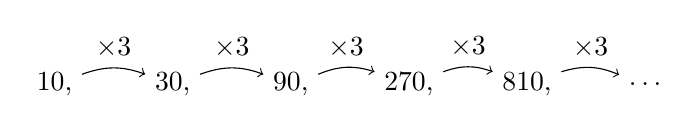
\begin{tikzpicture}[node distance=1.5cm]
    \node (a1) {$10$,};
    \node (a2) [right of=a1] {$30$,};
    \node (a3) [right of=a2] {$90$,};
    \node (a4) [right of=a3] {$270$,};
    \node (a5) [right of=a4] {$810$,};
    \node (a6) [right of=a5] {$\ldots$};

    \path[->] (a1) edge [bend left=20] node[above] {$\times 3$} (a2);
    \path[->] (a2) edge [bend left=20] node[above] {$\times 3$} (a3);
    \path[->] (a3) edge [bend left=20] node[above] {$\times 3$} (a4);
    \path[->] (a4) edge [bend left=20] node[above] {$\times 3$} (a5);
    \path[->] (a5) edge [bend left=20] node[above] {$\times 3$} (a6);
  \end{tikzpicture}
\end{image}
Let's see a graph: 
\begin{image}
\begin{tikzpicture}
	\begin{axis}[
            domain=0:6,xmin=0,xmax=6,ymin=-100,ymax=900,
            width=4in,
            height=2in,
            xtick={1,2,...,5},
            ytick={10,30,90,270,810},
            yticklabels={},%$a_1 = 10$,$a_2=30$,$a_3=90$,$a_4=270$,$a_5=810$},
            axis lines =middle, xlabel=$n$, ylabel=$a$,
            every axis y label/.style={at=(current axis.above origin),anchor=south},
            every axis x label/.style={at=(current axis.right of origin),anchor=west},
            clip=false,
            %axis on top,
          ]
          \addplot[color=penColor,fill=penColor,only marks,mark=*] coordinates{(1,10)};  %% closed hole          
          \addplot[color=penColor,fill=penColor,only marks,mark=*] coordinates{(2,30)};  %% closed hole          
          \addplot[color=penColor,fill=penColor,only marks,mark=*] coordinates{(3,90)};  %% closed hole          
          \addplot[color=penColor,fill=penColor,only marks,mark=*] coordinates{(4,270)};  %% closed hole          
          \addplot[color=penColor,fill=penColor,only marks,mark=*] coordinates{(5,810)};  %% closed hole  
        \end{axis}
\end{tikzpicture}
\end{image}

If the common ratio of a geometric sequence is between $0$ and $1$, a
geometric sequence will decrease as it progresses.

\begin{image}
  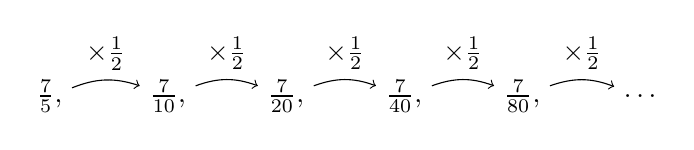
\begin{tikzpicture}[node distance=1.5cm]
    \node (a1) {$\frac{7}{5}$,};
    \node (a2) [right of=a1] {$\frac{7}{10}$,};
    \node (a3) [right of=a2] {$\frac{7}{20}$,};
    \node (a4) [right of=a3] {$\frac{7}{40}$,};
    \node (a5) [right of=a4] {$\frac{7}{80}$,};
    \node (a6) [right of=a5] {$\ldots$};
    
    \path[->] (a1) edge [bend left=20] node[above] {$\times\frac{1}{2}$} (a2);
    \path[->] (a2) edge [bend left=20] node[above] {$\times\frac{1}{2}$} (a3);
    \path[->] (a3) edge [bend left=20] node[above] {$\times\frac{1}{2}$} (a4);
    \path[->] (a4) edge [bend left=20] node[above] {$\times\frac{1}{2}$} (a5);
    \path[->] (a5) edge [bend left=20] node[above] {$\times\frac{1}{2}$} (a6);
  \end{tikzpicture}
\end{image}
Let's see a graph:
\begin{image}
\begin{tikzpicture}
	\begin{axis}[
            domain=0:6,xmin=0,xmax=6,ymin=0,ymax=2,
            width=4in,
            height=2in,
            xtick={1,2,...,5},
            ytick={1.4,.7,.35,.175,.0875},
            yticklabels={},%$a_1 = 10$,$a_2=30$,$a_3=90$,$a_4=270$,$a_5=810$},
            axis lines =middle, xlabel=$n$, ylabel=$a$,
            every axis y label/.style={at=(current axis.above origin),anchor=south},
            every axis x label/.style={at=(current axis.right of origin),anchor=west},
            clip=false,
            %axis on top,
          ]
          \addplot[color=penColor,fill=penColor,only marks,mark=*] coordinates{(1,7/5)};  %% closed hole          
          \addplot[color=penColor,fill=penColor,only marks,mark=*] coordinates{(2,7/10)};  %% closed hole          
          \addplot[color=penColor,fill=penColor,only marks,mark=*] coordinates{(3,7/20)};  %% closed hole          
          \addplot[color=penColor,fill=penColor,only marks,mark=*] coordinates{(4,7/40)};  %% closed hole          
          \addplot[color=penColor,fill=penColor,only marks,mark=*] coordinates{(5,7/80)};  %% closed hole  
        \end{axis}
\end{tikzpicture}
\end{image}


\begin{question}
  When the common ratio between successive elements of a geometric sequence is positive, which
  type of curves below model geometric sequences?
  \begin{multipleChoice}
    \choice{lines}
    \choice{parabolas}
    \choice{polynomials}
    \choice[correct]{exponential curves}
  \end{multipleChoice}
  \begin{feedback}
  If a geometric sequence is expressed as $a_n = a_1 \cdot r^{n-1}$,
  then in function notation we have $a(x) = a_1 \cdot r^{x-1}$, an
  exponential function.
  \end{feedback}
\end{question}



On the other hand, if the common ration between successive elements of
a geometric sequence is \textbf{not} positive, then something
interesting happens. Check out this example:
\begin{image}
  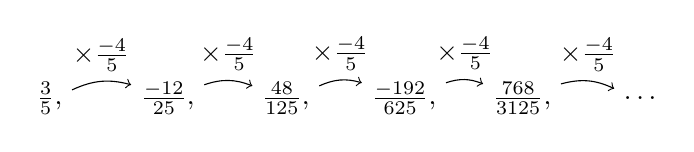
\begin{tikzpicture}[node distance=1.5cm]
    \node (a1) {$\frac{3}{5}$,};
    \node (a2) [right of=a1] {$\frac{-12}{25}$,};
    \node (a3) [right of=a2] {$\frac{48}{125}$,};
    \node (a4) [right of=a3] {$\frac{-192}{625}$,};L
    \node (a5) [right of=a4] {$\frac{768}{3125}$,};
    \node (a6) [right of=a5] {$\ldots$};
    
    \path[->] (a1) edge [bend left=20] node[above] {$\times\frac{-4}{5}$} (a2);
    \path[->] (a2) edge [bend left=20] node[above] {$\times\frac{-4}{5}$} (a3);
    \path[->] (a3) edge [bend left=20] node[above] {$\times\frac{-4}{5}$} (a4);
    \path[->] (a4) edge [bend left=20] node[above] {$\times\frac{-4}{5}$} (a5);
    \path[->] (a5) edge [bend left=20] node[above] {$\times\frac{-4}{5}$} (a6);
  \end{tikzpicture}
\end{image}
Let's see a graph:
\begin{image}
\begin{tikzpicture}
	\begin{axis}[
            domain=0:6,xmin=0,xmax=6,ymin=-.7,ymax=.7,
            width=4in,
            height=2in,
            xtick={1,2,...,5},
            ytick={.6,-.48,.384,-.3072,.24576},
            yticklabels={},%$a_1 = 10$,$a_2=30$,$a_3=90$,$a_4=270$,$a_5=810$},
            axis lines =middle, xlabel=$n$, ylabel=$a$,
            every axis y label/.style={at=(current axis.above origin),anchor=south},
            every axis x label/.style={at=(current axis.right of origin),anchor=west},
            clip=false,
            %axis on top,
          ]
          \addplot[color=penColor,fill=penColor,only marks,mark=*] coordinates{(1,3/5)};  %% closed hole          
          \addplot[color=penColor,fill=penColor,only marks,mark=*] coordinates{(2,-12/25)};  %% closed hole          
          \addplot[color=penColor,fill=penColor,only marks,mark=*] coordinates{(3,48/125)};  %% closed hole          
          \addplot[color=penColor,fill=penColor,only marks,mark=*] coordinates{(4,-192/625)};  %% closed hole          
          \addplot[color=penColor,fill=penColor,only marks,mark=*] coordinates{(5,768/3125)};  %% closed hole  
        \end{axis}
\end{tikzpicture}
\end{image}
The sign of this sequence alternates! 

\begin{warning}

There is a connection between sequences and functions,  but a little care must be taken.  Many different functions can agree when they are evaluated at the integers.

\begin{example}
Consider $a_n = 2n+1$ and the functions $f(x) = 2x+1$ and $g(x) = \frac{2x+1}{4}(4+\sin(\pi x))$.  The graphs of each are shown below:

\begin{image}
\begin{tikzpicture}
	\begin{axis}[
            domain=.8:6.5,xmin=0,xmax=6.5,ymin=-1,ymax=15,
            width=4in,
            height=2in,
            axis lines =middle, xlabel=$x$, ylabel=$y$,
            xtick={1,2,...,6},
            ytick={3,5,7,9,11,13},
            yticklabels={$a_1 = 3$,$a_2=5$,$a_3=7$,$a_4=9$,$a_5=11$,$a_6=13$},
            every axis y label/.style={at=(current axis.above origin),anchor=south},
            every axis x label/.style={at=(current axis.right of origin),anchor=west},
            clip=false,
            %axis on top,
          ]
       
           \addplot [penColor5,very thick,smooth,domain=.2:6.5]{2*x+1};
          \addplot [penColor6,very thick,smooth,domain=.2:6.2,samples=300]{(2*x+1)*(1+.25*sin(deg(2*pi*x)))};
          \addplot[color=penColor,fill=penColor,only marks,mark=*,ultra thick] coordinates{(1,3)};  %% closed hole        
          \addplot[color=penColor,fill=penColor,only marks,mark=*,ultra thick] coordinates{(2,5)};  %% closed hole        
          \addplot[color=penColor,fill=penColor,only marks,mark=*,ultra thick] coordinates{(3,7)};  %% closed hole        
          \addplot[color=penColor,fill=penColor,only marks,mark=*,ultra thick] coordinates{(4,9)};  %% closed hole        
          \addplot[color=penColor,fill=penColor,only marks,mark=*,ultra thick] coordinates{(5,11)};  %% closed hole    
          \addplot[color=penColor,fill=penColor,only marks,mark=*,ultra thick] coordinates{(6,13)};  %% closed hole         
        \end{axis}
\end{tikzpicture}
\end{image}

Note that if $n$ is a positive integer:

\begin{itemize}
\item $f(n) = 2n+1$.
\item Since $\sin(k \pi) = \answer{0}$ for all integers $k$, $g(n) = \frac{2n+1}{4}(4+\sin(n \pi)) = \frac{2n+1}{\cancel{4}}(\cancel{4}) = 2n+1$.
\end{itemize}

It should not be too surprising that several functions can be used to represent the same sequence because the sequence is defined only for \emph{discretely} many values, while the functions above are defined for \emph{all} real $x$-values. 
\end{example}

\end{warning}

It is very useful to associate the most ``obvious'' function to a given sequence when possible.  To do this for a given sequence $a_n$, we can try replacing the variable $n$ in the formula with $x$ and let $f(x)$ be the function obtained this way.

\begin{question}
  Using the convention above, which function corresponds to the sequence given by the explicit formula
  $a_n = -n/2+3$ for $n=1,2,3,\dots$?
  \begin{prompt}
    \[
    a(x) = \answer[given]{-x/2 + 3}
    \]
  \end{prompt}
\end{question}

\begin{warning}
This is not always as straight forward as above.  For instance, if $a_n = \frac{(-1)^n}{n}$, we cannot set $f(x) = \frac{(-1)^x}{x}$ because this function is real-valued for all real $x$.
\end{warning}

Since sequences can be conceptualized as functions, and calculus is
used to study functions, we can now apply our knowledge of calculus to
sequences!


\section{Limits of sequences}
Since sequences are essentially \dfn{discrete}, meaning that the points
are separate and distinct, the notion of a ``limit at a point'' cannot
be made to really make sense. However, limits at \textit{infinity} are
a different story.

In short, given a sequence, it is helpful to be able to say something
qualitative about it; we may want to address the question such as
``what happens after a while?'' 

Earlier, you've studied a similar question about
\[
\lim_{x\to\infty} f(x)
\]
when $x$ is a variable taking on real values; now, we simply want to
restrict the ``input'' values to be integers.  We have previously studied how to compute limits like the one above, so the curious young mathematician could certainly ask whether the old techniques for functions can still can be applied to find limits of sequences.

Note that there is not a perfect parallel between limits of functions and limits of sequences, as illustrated by the following example:

\begin{example}
  Let $a_n = \sin(n\pi)$ and $f(x) = \sin(\pi x)$. Show that
  \[
  \lim_{n\to\infty} a_n \ne \lim_{x\to \infty}f(x).
  \]
  \begin{explanation}
  The sequence $\{a_n\}_{n=1}^{\infty}$ is the ordered  list of numbers:
  \[
  \sin(0\pi),\, \sin(1\pi),\, \sin(2\pi),\,\sin(3\pi),\,\ldots
  \]
Since $\sin(n\pi)=0$, this list is actually:
  \[
  0,\, 0 , \, 0 ,\,0,\,\ldots
  \]
whenever $n$ is an integer.  Since every term in the sequence is $0$, we have:
\[
\lim_{n\to\infty} a_n = 0. 
\]
But $\lim_{x\to\infty}f(x)$, when $x$ is real, does not exist: as $x$
gets arbitrarily large, the values $\sin(x\pi)$ do not get closer and
closer to a single value, but instead oscillate between $-1$ and $1$.

This is shown graphically below:

\begin{image}
\begin{tikzpicture}
	\begin{axis}[
            domain=.8:6.5,xmin=0,xmax=6.5,ymin=-1.5,ymax=1.5,
            width=4in,
            height=2in,
            axis lines =middle, xlabel=$x$, ylabel=$y$,
            xtick={1,2,...,6},
            ytick={-1,1},
            every axis y label/.style={at=(current axis.above origin),anchor=south},
            every axis x label/.style={at=(current axis.right of origin),anchor=west},
            clip=false,
            %axis on top,
          ]
       
          \addplot [penColor5,very thick,smooth,domain=.2:6.2,samples=300]{sin(deg(pi*x)))};
          \addplot[color=penColor,fill=penColor,only marks,mark=*,ultra thick] coordinates{(1,0)};  %% closed hole        
          \addplot[color=penColor,fill=penColor,only marks,mark=*,ultra thick] coordinates{(2,0)};  %% closed hole        
          \addplot[color=penColor,fill=penColor,only marks,mark=*,ultra thick] coordinates{(3,0)};  %% closed hole        
          \addplot[color=penColor,fill=penColor,only marks,mark=*,ultra thick] coordinates{(4,0)};  %% closed hole        
          \addplot[color=penColor,fill=penColor,only marks,mark=*,ultra thick] coordinates{(5,0)};  %% closed hole    
          \addplot[color=penColor,fill=penColor,only marks,mark=*,ultra thick] coordinates{(6,0)};  %% closed hole         
        \end{axis}
\end{tikzpicture}
\end{image}


  \end{explanation}
\end{example}

The preceding example illustrates that:

\begin{multipleChoice}
\choice{If $\lim_{n \to \infty} a_n$ exists, then $\lim_{x \to \infty} f(x)$ exists.}
\choice{If  $\lim_{x \to \infty} f(x)$ does not exist, then $\lim_{n \to \infty} a_n$ does not exist.}
\choice[correct]{If $\lim_{x \to \infty} f(x)$ does not exist, $\lim_{n \to \infty} a_n$ may still exist.}
\end{multipleChoice}

This might lead us to believe that we need to develop a whole new arsenal of techniques in order to determine if limits of sequences exist, but there is good news:

\begin{theorem}
  Let $\{a_n\}$ be a sequence and suppose that $f(x)$ is a real-valued function for which $f(n) = a_n$ for all integers $n$.  If
  \[
  \lim_{x\to\infty}f(x)=L,
  \]
  then $\lim_{n\to\infty} a_n=L$ as well.
\end{theorem}

\begin{warning}
Remember that the converse of this theorem is not
true.  In the example preceding this theorem, have an explicit example of a function $f(x)$ and a sequence $(a_n)$ where $a_n
=f(n)$ and
\[
\lim_{x\to\infty}f(x)=\text{DNE} \quad\text{but} \quad \lim_{n\to\infty} a_n = 0.
\]

\end{warning}

If we think about the theorem a bit further, the conclusion  of the theorem and the content of the preceding example should seem reasonable.  If the values of $f(x)$ become arbitrarily close to a number $L$ for \emph{all} arbitrarily large $x$, then the result should still hold when we only consider \emph{some} of these values.  However, if we only know what happens for \emph{some} arbitrarily large $x$-values, we cannot say what happens for \emph{all} of them!

%
%Here is some general advice. If you want to know $\lim_{n\to\infty}
%a_n$, you might first think of a function $f(x)$ where $a_n = f(n)$,
%and then attempt to compute $\lim_{x\to\infty}f(x)$.  If the limit of
%the function exists, then it is equal to the limit of the sequence.
%But, if for some reason $\lim_{x\to\infty}f(x)$ does not exist, it may
%nevertheless still be the case that $\lim_{n\to\infty}a_n$ exists,
%you'll just have to figure out another way to compute it.

%%%%%%%%%%%%%THE COMMENTED MATERIAL BELOW IS DANGEROUS; AN IMPORTANT POINT IN THE PRECEDING SECTION IS THAT THERE IS A DIFFERENCE BETWEEN THE LIST AND THE RULE THAT GENERATES IT.  WE SHOULD NOT BE PURPOSEFULLY ENCOURAGING STUDENTS TO CONFLATE CLASSES OF OBJECTS IN A CHAPTER THAT REALLY REQUIRES THEM TO CRYSTALLIZE DEFINITIONS AND CONCEPTS%%%%%%%%%%%%%%%%%%%

%Let's summarize the preceding section in the following formal definition.
%\begin{definition}
%  A \dfn{sequence} $\{a_n\}_{n=N}$ is an order list that is generated by a real-valued
%  function $f:D \to \R$, where $D = \{ N, N+1, N+2, \ldots \}$ is the domain of the function
%  \]
%\end{definition}
%
%Stated more humbly, a sequence assigns a unique real number to each of the integers
%starting with an index $N$.
%
%When thought of as a function, the ``outputs'' of a sequence are the
%\dfn{elements} of the sequence; the ``$n$th element'' is the real
%number that the sequence associates to the natural number $n$, and is
%usually written $a_n$. \index{sequence!element} The $n$ in the phrase
%``$n$th element'' is called an \dfn{index}\index{sequence!index}; the
%plural of index is either indices or indexes, depending on who you
%ask.  The first index $N$ is called the \dfn{initial index}. 


%%%%%%%%%%%%%%%%%%%%%%%%%%%%%%%%%%%%%%%%%%%%%%%%%%%%



%\section{Plotting sequences}<------ARITHMETIC TO EXERCISES?
%
%First, we plot sequences as points. Later, we will see another
%interpretation.
%
%\subsection{Plots of arithmetic sequences}
%
%Recall that arithmetic sequences are those where the difference
%between neighboring elements is constant.  Arithmetic sequences are
%analogues of lines.  Consider a basic example:
%\begin{image}
%  \begin{tikzpicture}[node distance=1.5cm]
%    \node (a1) {$-5$,};
%    \node (a2) [right of=a1] {$-1$,};
%    \node (a3) [right of=a2] {$3$,};
%    \node (a4) [right of=a3] {$7$,};
%    \node (a5) [right of=a4] {$11$,};
%    \node (a6) [right of=a5] {$\ldots$};
%    
%    \path[->] (a1) edge [bend left=20] node[above]{$+4$} (a2);
%    \path[->] (a2) edge [bend left=20] node[above]{$+4$} (a3);
%    \path[->] (a3) edge [bend left=20] node[above]{$+4$} (a4);
%    \path[->] (a4) edge [bend left=20] node[above]{$+4$} (a5);
%    \path[->] (a5) edge [bend left=20] node[above]{$+4$} (a6);
%  \end{tikzpicture}
%\end{image}
%
%Check out a graph of the sequence:
%
%\begin{image}
%\begin{tikzpicture}
%	\begin{axis}[
%            domain=0:6,xmin=0,xmax=6,ymin=-9,ymax=15,
%            width=4in,
%            height=2in,
%            axis lines =middle, xlabel=$n$, ylabel=$a$,
%            xtick={1,2,...,5},
%            ytick={-5,-1,...,11},
%            yticklabels={$a_1 = -5$,$a_2=-1$,$a_3=3$,$a_4=7$,$a_5=11$},
%            every axis y label/.style={at=(current axis.above origin),anchor=south},
%            every axis x label/.style={at=(current axis.right of origin),anchor=west},
%            clip=false,
%            %axis on top,
%          ]
%          \addplot[color=penColor,fill=penColor,only marks,mark=*] coordinates{(1,-5)};  %% closed hole          
%          \addplot[color=penColor,fill=penColor,only marks,mark=*] coordinates{(2,-1)};  %% closed hole          
%          \addplot[color=penColor,fill=penColor,only marks,mark=*] coordinates{(3,3)};  %% closed hole          
%          \addplot[color=penColor,fill=penColor,only marks,mark=*] coordinates{(4,7)};  %% closed hole          
%          \addplot[color=penColor,fill=penColor,only marks,mark=*] coordinates{(5,11)};  %% closed hole  
%        \end{axis}
%\end{tikzpicture}
%\end{image}
%
%Here is an arithmetic sequence that decreases as its index increases.
%
%\begin{image}
%  \begin{tikzpicture}[node distance=1.5cm]
%    \node (a1) {$17$,};
%    \node (a2) [right of=a1] {$15$,};
%    \node (a3) [right of=a2] {$13$,};
%    \node (a4) [right of=a3] {$11$,};
%    \node (a5) [right of=a4] {$9$,};
%    \node (a6) [right of=a5] {$\ldots$};
%
%    \path[->] (a1) edge [bend left=20] node[above]{$-2$} (a2);
%    \path[->] (a2) edge [bend left=20] node[above]{$-2$} (a3);
%    \path[->] (a3) edge [bend left=20] node[above]{$-2$} (a4);
%    \path[->] (a4) edge [bend left=20] node[above]{$-2$} (a5);
%    \path[->] (a5) edge [bend left=20] node[above]{$-2$} (a6);
%  \end{tikzpicture}
%\end{image}
%
%Here we see a graph:
%
%\begin{image}
%\begin{tikzpicture}
%	\begin{axis}[
%            domain=0:6,xmin=0,xmax=6,ymin=7,ymax=19,
%            width=4in,
%            height=2in,
%            xtick={1,2,...,5},
%            ytick={17,15,...,9},
%            yticklabels={$a_1 = 17$,$a_2=15$,$a_3=13$,$a_4=11$,$a_5=9$},
%            axis lines =middle, xlabel=$n$, ylabel=$a$,
%            every axis y label/.style={at=(current axis.above origin),anchor=south},
%            every axis x label/.style={at=(current axis.right of origin),anchor=west},
%            clip=false,
%            %axis on top,
%          ]
%          \addplot[color=penColor,fill=penColor,only marks,mark=*] coordinates{(1,17)};  %% closed hole          
%          \addplot[color=penColor,fill=penColor,only marks,mark=*] coordinates{(2,15)};  %% closed hole          
%          \addplot[color=penColor,fill=penColor,only marks,mark=*] coordinates{(3,13)};  %% closed hole          
%          \addplot[color=penColor,fill=penColor,only marks,mark=*] coordinates{(4,11)};  %% closed hole          
%          \addplot[color=penColor,fill=penColor,only marks,mark=*] coordinates{(5,9)};  %% closed hole  
%        \end{axis}
%\end{tikzpicture}
%\end{image}
%
%
%\begin{question}
%  To what type of curve do arithmetic sequences correspond?
%  \begin{multipleChoice}
%    \choice[correct]{lines}
%    \choice{parabolas}
%    \choice{polynomials}
%    \choice{exponential curves}
%    \choice{impossible to say}
%  \end{multipleChoice}
%  \begin{feedback}
%    Since the average growth rate of a line is constant regardless of
%    the size of the interval chosen, arithmetic sequences correspond to
%    lines.
%  \end{feedback}
%\end{question}
%

\begin{example}
Let $a_n = \frac{5n+1}{6n+7}$.  Determine if the sequence $\{a_n\}_{n=1}^{\infty}$ has a limit.

\begin{explanation}
A function that can be used to generate the sequence is $f(x) = \frac{5x+1}{6x+7}$.  Since $\lim_{x \to \infty} \frac{5x+1}{6x+7} = \answer[given]{\frac{5}{6}}$, we have:

\[
\lim_{n \to \infty} a_n = \answer[given]{\frac{5}{6}}
\]
\end{explanation}

\end{example}

\section{Computing limits of sequences using dominant term analysis}
The last example shows us that for many sequences, we can employ the same techniques that we used to compute limits previously.  While algebraic techniques and L'Hopital's rule are useful, in many of the following sections, being able to determine limits quickly is an important skill.  In order to do this, we have to become good at recognizing the terms in a given sequence that ultimately determine whether its limit exists.

\begin{example}
Let $a_n = \frac{n^3+4n^2-1}{2-4n^4}$.  Determine if the limit of the sequence $\{a_n\}_{n=1}^{\infty}$ exists.

\begin{explanation}
The highest degree term in the numerator is $n^3$, while the largest term in the denominator is $-4n^4$.  We can do a little algebra:

\[
\frac{n^3+4n^2-1}{2-4n^3} = \frac{n^3\left(1+\frac{4}{n}-\frac{1}{n^3}\right)}{-4n^4\left(-\frac{1/2}{n^4}+1\right)} = \frac{n^3}{-4n^4} \cdot  \frac{1+\frac{4}{n}-\frac{1}{n^3}}{-\frac{1/2}{n^4}+1}
\]
The second term becomes arbitrarily close to $1$ as $n$ grows larger and larger, so the limit of the sequence is completely determined by the ratio of the highest degree term in the numerator to the highest degree term in the denominator.  In this case, that ratio is $\frac{n^3}{-4n^4} = \frac{1}{-4n}$, so $\lim_{n \to \infty} a_n = 0$.

\end{explanation}
\end{example}

\begin{remark}
In the preceding example, we say that the \emph{dominant term} in the numerator is $n^3$ and that the \emph{dominant term} in the denominator is $-4n^4$ because these terms are the only ones that are relevant when finding the limit.
\end{remark}

Sometimes, this can be used to find limits where L'Hopital's rule or an algebraic approach would be complicated.

\begin{example}
Let $a_n = \frac{n^2(2n+1)(5-3n)}{(1+2n)^4}$.  Determine if the limit of the sequence $\{a_n\}_{n=1}^{\infty}$ exists.

\begin{explanation}
The dominant term in the numerator is $n^2 \cdot 2n \cdot (-3n) = \answer{-6n^4}$, while the dominant term in the denominator is $(2n)^4 = \answer{16}n^4$.  By noting that:

\[
\lim_{n \to \infty} \frac{-6n^4}{16n^4} = \answer{-\frac{6}{16}},
\]
we find $\lim_{n \to \infty} a_n = \answer{-\frac{6}{16}}$.
\end{explanation}
\end{example}
 
\subsection{Growth rates}
The preceding examples illustrate that higher positive powers of $n$ grow more quickly than lower positive powers of $n$.  We can introduce a little notation that captures this in a succinct way:

\begin{definition}
  Given two sequences $(a_n)$ and $(b_n)$, the notation $(a_n) \ll
  (b_n)$ means that
  \[
  \lim_{n\to\infty} \frac{a_n}{b_n} =
  0\qquad\text{and}\qquad\lim_{n\to\infty} \frac{b_n}{a_n} =\infty.
  \]
\end{definition}

In essence, writing $a_n \ll b_n$ says that the sequence $(b_n)$ grows
much faster than $(a_n)$.

\begin{example}
Suppose that $a_n = 4n^2+3n$ and $b_n = 5n^{3/2}+2n$.  Then, we can compute $\lim_{n \to \infty} \frac{a_n}{b_n} = \answer{\infty}$ and $\lim_{n \to \infty} \frac{b_n}{a_n} = \answer{0}$.  We thus write:

\begin{multipleChoice}
\choice{$a_n  \ll b_n$}
\choice[correct]{$b_n  \ll a_n$}
\end{multipleChoice}

\end{example}

Many sequences of interest involve terms other than powers of $n$.  It is often useful to understand how different \emph{types} of functions grow relative to each other:

\begin{theorem}[Growth rates of sequences]
  Let $p,q$ be positive real numbers, and let $b> 1$. We have the
  following relationship:
  \[
  (\ln^p(n))\ll (n^q) \ll (b^n) \ll (n!) \ll (n^n)
  \]
\end{theorem}

The first inequality in this theorem essentially guarantees that \emph{any} power of $\ln(n)$ grows more slowly than \emph{any} power of $n$.  For example: 

\begin{example}
  Let $a_n  = \frac{\ln^{9}(n)}{n^{1/2}}$.  What is $\lim_{n \to \infty} a_n$?
  
  \begin{explanation}
  By growth rates, $\lim_{n\to\infty}a_n =\answer[given]{0}$.  
  
  \end{explanation}
\end{example}

This allows us to extend the \emph{dominant term} idea to more complicated expressions:

\begin{example}
  Let $a_n  = \frac{n^{100} + n^n}{n!+5^n}$.  What is $\lim_{n \to \infty} a_n$?
  
  \begin{explanation}
  By growth rates, the dominant term in the numerator is $n^n$, and the dominant term in the denominator is $n!$.  We thus will know if $\lim_{n \to \infty} a_n$ exists by considering $\lim_{n \to \infty} \frac{n^n}{n!}$.  By growth rates, this limit is infinite, so $\lim_{n \to \infty} a_n = \infty$.
  
  \end{explanation}
\end{example}

%%%%%%%%%%%%%%%%%%%%%%%%%%%%%%%%%%%%%%%%
\subsection{The squeeze theorem}

Previously, when considering limits, one of our techniques was to replace 
complicated functions by simpler functions. The \textit{Squeeze Theorem}
tells us one situation where this is possible.

\begin{theorem}[Squeeze Theorem]\index{Squeeze Theorem}
  Suppose that $(a_n)$, $(b_n)$, and $(c_n)$ are sequences with
  \[
  a_n \le b_n \le c_n
  \]
  for all $n$ greater than some index $N$. If
  \[
  \lim_{n\to\infty} a_n = L = \lim_{n\to\infty} c_n,
  \] 
  then $\lim_{n\to\infty} b_n = L$.
\end{theorem}

Let's see an example.

\begin{example}
  Consider the sequence $(b_n)_{n=1}^{\infty}$ where $b_n =
  \left(\frac{-1}{2}\right)^n$. Compute:
  \[
  \lim_{n\to\infty}b_n
  \]
  \begin{explanation}
    To compute this limit we will use the squeeze theorem. Write with
    me:
    \[
    -\left(\frac{1}{2}\right)^n\le \left(\frac{-1}{2}\right)^n \le \left(\frac{1}{2}\right)^n
    \]
    but we know
    \[
    \lim_{n\to \infty}\left(-\left(\frac{1}{2}\right)^n\right) = \answer[given]{0}
    \]
    and
    \[
    \lim_{n\to \infty}\left(\frac{1}{2}\right)^n =\answer[given]{0}.
    \]
    Hence by the squeeze theorem, $\lim_{n\to\infty} b_n = \answer[given]{0}$.
  \end{explanation}
\end{example}


This last result actually gives us a general theorem about geometric
sequences:

\begin{theorem}
  Given a geometric sequence $a_n = a_1 \cdot r^{n-1}$,
  \[
  \lim_{n\to\infty} a_n =
  \begin{cases}
    0 &\text{if $|r|<1$,}\\
    1 &\text{if $r=1$,}\\
    \text{DNE} &\text{if $|r|>1$ or $r=-1$.}
  \end{cases}
  \]
\end{theorem}

%%%%%%%%%%%%%%%%%%%%%%%%%%%%%%%%%%%%%%%%

\subsection{The monotone convergence theorem}

Perhaps the ``best" way to determine whether the limit of a sequence exists is to compute it, but this is not always feasible if we only have a recursive description of a sequence rather than an explicit one.  In fact, in many of the coming sections, this is all we will have easily, so we want to determine a good approach for determining whether a limit exists without having to compute it directly.  To do this, we introduce some terminology focused on the relationships between the terms of a sequence.

\begin{definition}
  A sequence is called
  \begin{itemize}
    \item \dfn{increasing} if $a_n<a_{n+1}$ for all $n$,
    \item \dfn{nondecreasing} if $a_n\le a_{n+1}$ for all $n$,
    \item \dfn{decreasing} if $a_n>a_{n+1}$ for all $n$,
    \item \dfn{nonincreasing} if $a_n\ge a_{n+1}$ for all $n$.
  \end{itemize}
\end{definition}

Lots of facts are true for sequences which are either increasing or
decreasing; to talk about this situation without constantly saying
``either increasing or decreasing,'' we can introduce a single word to
cover both cases.
\begin{definition}
  If a sequence is always increasing, or  always nondecreasing, or always decreasing, or always nonincreasing, it is said to be \dfn{monotonic}\index{sequence!monotonic}.
\end{definition}


\begin{example}
If $a_n = 2n^2+1$, then $\{a_n\}_{n=1}^{\infty}$ is \wordChoice{\choice[correct]{increasing}\choice{decreasing}}, so it is
      \wordChoice{\choice[correct]{monotonic}\choice{not monotonic}}
\end{example}

\begin{question}
  If an arithmetic sequence $a_n = m\cdot n + b$ is monotonic, what
  must be true about $m$ and $b$?
  \begin{prompt}
    \begin{quote}
      The sign of $m$ \wordChoice{\choice{is positive}\choice{is
          negative}\choice[correct]{does not matter}}, and the sign of $b$ is
      \wordChoice{\choice{is positive}\choice{is negative}\choice[correct]{does
          not matter}}
    \end{quote}
  \end{prompt}
  \begin{feedback}
    An arithmetic sequence is always monotonic, regardless of the
    values of $m$ and $b$.
  \end{feedback}
\end{question}

\begin{question}
  If a geometric sequence $a_n = a_1 \cdot r^{n-1}$ is monotonic, what
  must be true about $a_1$ and $r$?
  \begin{prompt}
    \begin{quote}
      The sign of $a_1$ \wordChoice{\choice{is positive}\choice{is
          negative}\choice[correct]{does not matter}}, and the sign of
      $r$ is \wordChoice{\choice[correct]{is positive}\choice{is
          negative}\choice{does not matter}}
    \end{quote}
  \end{prompt}
    \begin{feedback}
    A geometric sequence $a_n = a_1 \cdot r^{n-1}$ is monotonic if and
    only if the sign of $r$ is positive.
  \end{feedback}
\end{question}

%Let's see some examples:
%\begin{example}
%  Describe the growth of $a_n = \frac{2^n-1}{2^n}$ for
%  $n=1,2,3,\dots$.
%  \begin{explanation}
%    To do this, check out the difference between two sequential terms,
%    write with me:
%    \begin{align*}
%    a_{n+1} - a_n &= \answer[given]{\frac{2^{n+1}-1}{2^{n+1}}} - \frac{2^n-1}{2^n}\\
%    &=\frac{2^{n+1}-1 - 2\left(\answer[given]{2^n-1}\right)}{2^{n+1}}\\
%    &=\frac{2^{n+1}-1 - 2^{n+1}+2}{2^{n+1}}\\
%    &=\frac{\answer[given]{1}}{2^{n+1}}.
%    \end{align*}
%    Since $\frac{1}{2^{n+1}}$ is always
%    \wordChoice{\choice[correct]{positive}\choice{negative}\choice{zero}},
%    we see that $(a_n)$ is
%    \wordChoice{\choice[correct]{increasing}\choice{nondecreasing}\choice{decreasing}\choice{nonincreasing}}, and hence is \wordChoice{\choice[correct]{monotonic}\choice{not monotonic}}.
%  \end{explanation}
%\end{example}
%
%\begin{example}
%  Describe the growth of $a_n = \frac{n+1}{n}$ for $n=1,2,3,\dots$.
%  \begin{explanation}
%    To do this, check out the difference between two sequential terms.
%    Write with me.
%    \begin{align*}
%    a_{n+1} - a_n &= \answer[given]{\frac{(n+1)+1}{n+1}} - \frac{n+1}{n}\\
%    &=\frac{n(n+2) - (n+1)(\answer[given]{n+1})}{n+1}\\
%    &=\frac{n^2+2n - n^2 -2n-1}{n+1}\\
%    &=\frac{\answer[given]{-1}}{n+1}.
%    \end{align*}
%    Since $\frac{-1}{n+1}$ is always
%    \wordChoice{\choice{positive}\choice[correct]{negative}\choice{zero}} for the values of $n$ we are considering,
%    we see that $(a_n)$ is
%    \wordChoice{\choice{increasing}\choice{nondecreasing}\choice[correct]{decreasing}\choice{nonincreasing}}, and hence is \wordChoice{\choice[correct]{monotonic}\choice{not monotonic}}.
%  \end{explanation}
%\end{example}

Sometimes we want to classify whether the terms in the sequence do not get too big or too
small, in this case we say the sequence is \textit{bounded}.

\begin{definition}
  \label{definition:sequence-bounded}
  A sequence $\{a_n\}$ is:
  
  \begin{itemize}
  \item \dfn{bounded above} if there is some number $M$ so
  that for all $n$, we have $a_n\le M$.
    \item \dfn{bounded below} if there is some number $m$ so
  that for all $n$, we have $a_n\ge m$.
  \item \dfn{bounded} if it is both bounded above and bounded below.
  \end{itemize}
\end{definition}

So what does this actually say? Essentially, we say that a sequence is bounded above if its terms cannot become too large, bounded below if its terms cannot become too negative, and bounded if the terms cannot become too large or too negative.

\begin{question}
  True or False: If a sequence $(a_n)_{n=0}^\infty$ is nondecreasing
  it is bounded below by $a_0$.
  \begin{prompt}
    \begin{multipleChoice}
    \choice[correct]{True}
    \choice{False}
    \end{multipleChoice}
  \end{prompt}
  \begin{feedback}
    If a sequence is nondecreasing, then its smallest value is its
    first element.
  \end{feedback}
\end{question}


\begin{question}
  True or False: If a sequence $(a_n)_{n=0}^\infty$ is nonincreasing
  it is bounded above by $a_0$.
  \begin{prompt}
    \begin{multipleChoice}
    \choice[correct]{True}
    \choice{False}
    \end{multipleChoice}
  \end{prompt}
  \begin{feedback}
    If a sequence is nonincreasing, then its largest value is its
    first element.
  \end{feedback}
\end{question}

So, what do these terms have to do with the idea of a limit?  Essentially, there are three reasons that a sequence may diverge:

\begin{itemize}
\item The terms become too arbitrarily large or too negative.
\item The terms oscillate.
\item The terms oscillate and become both too large and too negative. 
\end{itemize}

Let's think about the terminology we introduced.

\begin{question}
\begin{itemize}
\item If we know that a sequence is monotonic and its limit does not exist, then  \wordChoice{\choice[correct]{the terms become too arbitrarily large or too negative}\choice{the terms oscillate}\choice{the terms oscillate and become both too large and too negative}}.

\item If we know that a sequence is bounded and its limit does not exist, then  \wordChoice{\choice{the terms become too arbitrarily large or too negative.}\choice[correct]{the terms oscillate}\choice{the terms oscillate and become both too large and too negative}}.

\end{itemize}
\end{question}

We can now state an important theorem:

\begin{theorem}[Bounded-monotone convergence theorem]
  If the sequence $a_n$ is bounded and monotonic, then $\lim_{n \to  \infty} a_n $ exists.
\end{theorem}

To think about the statement of the theorem, if we have a sequence that is bounded, the only way it could diverge is if the terms oscillate.  However, if we know the sequence is also monotonic, this cannot happen!  Thus, the series cannot diverge, so it must have a limit.

%\begin{question}
%  Consider the sequence $a_{n}$.  Suppose you know that for all $n >
%  1$,
%  \[
%  -6 \le a_{n} \le 0
%  \]
%  and $a_{1} = 2$, and $a_{2} = -1$, and that the sequence is
%  nonincreasing.  Does the sequence converge?
%  \begin{hint}
%    Since the sequence is nonincreasing, the sequence is monotone.
%  \end{hint}
%  \begin{hint}
%    Since for all $n \ge 1$, we have $a_{n} \ge -6$, the sequence is
%    bounded below.
%  \end{hint}
%  \begin{hint}
%    So by the Monotone Convergence Theorem, the sequence converges to
%    some value; let us call it $L$.
%  \end{hint}
%  \begin{hint}
%    Now consider the direction in which the sequence is heading.
%  \end{hint}
%  \begin{hint}
%    Since the sequence is nonincreasing, for all $n \ge 2$, we have
%    $-6 \le a_{n} \le -1$.
%  \end{hint}
%  \begin{hint}
%    The limit $L$ must be in that interval as well.
%  \end{hint}
%  \begin{hint}
%    Therefore the sequence converges to a value $L$ so that $-6 \le L
%    \le -1$.
%  \end{hint}
%  \begin{prompt}
%  \begin{multipleChoice}
%    \choice[correct]{Yes, with limit between $-6$ and $-1$.}
%    \choice{No, the sequence does not converge.}
%    \choice{Yes, with limit between $-1$ and $0$.}
%  \end{multipleChoice}
%  \end{prompt}
%\end{question}

In short, bounded monotonic sequences always converge, though we can't
necessarily describe the number to which they converge.  Let's try
some examples.

\begin{example}
  Given the sequence $a_n=\frac{2^n-1}{2^n}$ for $n=1,2,3,\dots$,
  explain how you know that $\lim_{n\to\infty} a_n$ converges to a
  finite value without computing its limit.
  \begin{explanation}
    To start, from previous work we know that $a_n$ is
    \wordChoice{\choice[correct]{monotonic}\choice{not monotonic}}.
    Moreover, all of the elements $a_n = (2^n-1)/2^n$ are less than
    $2$, and greater than zero. Hence by the bounded-monotone
    convergence theorem, $\lim_{n\to\infty} a_n$ converges to a finite
    value.
  \end{explanation}
\end{example}

%\begin{example}
%  Given the sequence $a_n=\frac{n+1}{n}$ for $n=1,2,3,\dots$,
%  explain how you know that $\lim_{n\to\infty} a_n$ converges to a
%  finite value.
%  \begin{explanation}
%    To start, from previous work we know that $a_n$ is
%    \wordChoice{\choice[correct]{monotonic}\choice{not monotonic}}.
%    Moreover, all of the elements $a_n = (n+1)/n$ are less than $2$,
%    and greater than zero. Hence by the bounded-monotone convergence
%    theorem, $\lim_{n\to\infty} a_n$ converges to a finite value.
%  \end{explanation}
%\end{example}

\begin{remark}
We don't actually need to know that a sequence is always monotonic to apply
the bounded-monotone convergence theorem. It is enough to know that
the sequence is ``eventually'' monotonic, that is, that some point it
becomes increasing or decreasing.
\end{remark}

%\begin{example}
%Show that the sequence $(a_n)$ given by $a_n = n^{1/n}$ converges.
%\begin{explanation}
%  We might first show that this sequence is decreasing, that is, we show
%  that for all $n$,
%  \[
%  n^{1/n} > (n+1)^{1/(n+1)}.
%  \]
%  But this isn't true!  Take a look
%  \begin{align*}
%    a_1 &= 1, \\
%    a_2 &= \sqrt{2} \approx 1.4142, \\
%    a_3 &= \sqrt[3]{3} \approx 1.4422, \\
%    a_4 &= \sqrt[4]{4} \approx 1.4142, \\
%    a_5 &= \sqrt[5]{5} \approx 1.3797, \\
%    a_6 &= \sqrt[6]{6} \approx 1.3480, \\
%    a_7 &= \sqrt[7]{7} \approx 1.3205, \\
%    a_8 &= \sqrt[8]{8} \approx 1.2968, \\
%    a_9 &= \sqrt[9]{9} \approx 1.2765.
%  \end{align*}
%  But it does seem that this sequence perhaps is decreasing after the
%  first few terms.  Can we justify this?
%
%  Yes!  Consider the real function $f(x)=x^{1/x}$ when $x\ge 1$.  We
%  compute the derivative, perhaps via \index{logarithmic
%    differentiation}logarithmic differentiation, to find
%  \[
%  f'(x)=\answer[given]{\frac{x^{1/x} (1-\ln(x))}{x^2}}.
%  \]
%  Note that when $x\ge 3$, the derivative $f'(x)$ is negative.  Since
%  the function $f$ is decreasing, we can conclude that the sequence is
%  decreasing---well, at least for $n \geq 3$.
%
%  Since all terms of the sequence are positive, the sequence is
%  decreasing and bounded $0\le a_n \le a_3$ when $n \ge 3$, and so the
%  sequence converges.
%\end{explanation}
%\end{example}

In the previous examples, we could write down a function $f(x)$ corresponding to each series and apply the theorem from earlier in the section.  However, this is not always possible.

\begin{example}
Suppose that $a_n = 2 + \sin(n)$, and let $s_n = \sum_{k=1}^{n} a_k$.  Determine whether the sequences $\{a_n\}$ and $\{s_n\}$ are bounded or monotonic, and explain whether either has a limit.

\begin{explanation}
The sequence $a_n$ is certainly not monotonic, but it  is bounded since $1 \geq a_n \geq 3$ for all $n$.  We also can see that $\lim_{n \to \infty} a_n$ does not exist since the terms oscillate.

For $s_n$, note that since $a_n \geq 1$ for all $n$, each term $a_n$ is positive.  Thus, $s_n$ is increasing and hence monotonic.  However, since $a_n\geq1$ for all $n$, we hav ethe following inequality:

\[s_n = \sum_{k=1}^n a_n \geq \sum_{k=1}^n 1 = n,\]

Hence, $\{s_n\}$ is not bounded.  Since $s_n$ is monotonic and not bounded, $\lim_{n \to \infty} s_n$ does not exist.
\end{explanation}
\end{example}

\begin{remark}
We had a way to compute analyze $\{a_n\}$ in the above example because we had an explicit formula for $a_n$, but how would we find such a formula for $s_n$?  As it turns out, we will study a more general case of this example in the coming sections, but we introduce it here to draw attention to the fact that many sequences of interest will not be described by a readily available explicit formula. 
\end{remark}



\end{document}
